\documentclass[11pt,a4paper]{ivoa}
\input tthdefs
%\usepackage[table]{xcolor}
%\usepackage{todonotes}

\usepackage{listings}
\definecolor{mygreen}{rgb}{0,0.6,0}
\definecolor{mygray}{rgb}{0.5,0.5,0.5}
\definecolor{mymauve}{rgb}{0.58,0,0.82}
\lstset{ %
  backgroundcolor=\color{white},   % choose the background color; you must add \usepackage{color} or \usepackage{xcolor}
  basicstyle=\footnotesize\ttfamily,        % the size of the fonts that are used for the code
  breakatwhitespace=false,         % sets if automatic breaks should only happen at whitespace
  breaklines=true,                 % sets automatic line breaking
  captionpos=b,                    % sets the caption-position to bottom
  commentstyle=\color{mygreen},    % comment style
  deletekeywords={...},            % if you want to delete keywords from the given language
  escapeinside={\%*}{*)},          % if you want to add LaTeX within your code
  extendedchars=true,              % lets you use non-ASCII characters; for 8-bits encodings only, does not work with UTF-8
  frame=single,                    % adds a frame around the code
  keepspaces=true,                 % keeps spaces in text, useful for keeping indentation of code (possibly needs columns=flexible)
  keywordstyle=\color{blue},       % keyword style
  language=Python,                 % the language of the code
  otherkeywords={*,...},            % if you want to add more keywords to the set
  numbers=left,                    % where to put the line-numbers; possible values are (none, left, right)
  numbersep=5pt,                   % how far the line-numbers are from the code
  numberstyle=\tiny\color{mygray}, % the style that is used for the line-numbers
  rulecolor=\color{black},         % if not set, the frame-color may be changed on line-breaks within not-black text (e.g. comments (green here))
  showspaces=false,                % show spaces everywhere adding particular underscores; it overrides 'showstringspaces'
  showstringspaces=false,          % underline spaces within strings only
  showtabs=false,                  % show tabs within strings adding particular underscores
  stepnumber=2,                    % the step between two line-numbers. If it's 1, each line will be numbered
  stringstyle=\color{mymauve},     % string literal style
  tabsize=2,                       % sets default tabsize to 2 spaces
  title=\lstname                   % show the filename of files included with \lstinputlisting; also try caption instead of title
}
% for large tables rotated in portrait format
\usepackage{rotating}
\usepackage{pdflscape}
\usepackage{lscape}

%multitable -)mir
\usepackage{subcaption}
\usepackage{tabularx}

\title{ObsCore Metadata Extension for Time Properties}

% see ivoatexDoc for what group names to use here; use \ivoagroup[IG] for
% interest groups.
\ivoagroup{DM}

\author[mireille.louys@unistra.fr]{Mireille Louys}
\author{Fran\c{c}ois Bonnarel}
\author{Vincenzo Galluzzi}
\author{Baptiste Cecconi}
\author{Ada Nebot}

\editor{Mireille Louys}

% \previousversion[????URL????]{????Concise Document Label????}
\previousversion{This is the first public release}

\begin{document}
\lstset{ %
  backgroundcolor=\color{white},   % choose the background color; you must add \usepackage{color} or \usepackage{xcolor}
  basicstyle=\footnotesize\ttfamily,        % the size of the fonts that are used for the code
  breakatwhitespace=false,         % sets if automatic breaks should only happen at whitespace
  breaklines=true,                 % sets automatic line breaking
  captionpos=b,                    % sets the caption-position to bottom
  commentstyle=\color{mygreen},    % comment style
  deletekeywords={...},            % if you want to delete keywords from the given language
  escapeinside={\%*}{*)},          % if you want to add LaTeX within your code
  extendedchars=true,              % lets you use non-ASCII characters; for 8-bits encodings only, does not work with UTF-8
  frame=single,                    % adds a frame around the code
  keepspaces=true,                 % keeps spaces in text, useful for keeping indentation of code (possibly needs columns=flexible)
  keywordstyle=\color{blue},       % keyword style
  language=Python,                 % the language of the code
  otherkeywords={*,...},            % if you want to add more keywords to the set
  numbers=left,                    % where to put the line-numbers; possible values are (none, left, right)
  numbersep=5pt,                   % how far the line-numbers are from the code
  numberstyle=\tiny\color{mygray}, % the style that is used for the line-numbers
  rulecolor=\color{black},         % if not set, the frame-color may be changed on line-breaks within not-black text (e.g. comments (green here))
  showspaces=false,                % show spaces everywhere adding particular underscores; it overrides 'showstringspaces'
  showstringspaces=false,          % underline spaces within strings only
  showtabs=false,                  % show tabs within strings adding particular underscores
  stepnumber=2,                    % the step between two line-numbers. If it's 1, each line will be numbered
  stringstyle=\color{mymauve},     % string literal style
  tabsize=2,                       % sets default tabsize to 2 spaces
  title=\lstname                   % show the filename of files included with \lstinputlisting; also try caption instead of title
}


\begin{abstract}
This IVOA specification details a list of metadata dealing with time-related features needed for  discovery 
of time series data sets, in the context of ObsTAP services.  
It is based on science cases explained in a previous IVOA note prepared in 2018 and recently revised \citep{note:TSSerialisationNote}.
Here we discuss various use-cases. 
We  highlight first which existing time related metadata in the ObsCore standard version 1.1 can be used, 
and second propose new features needed for an ObsCore time extension in order to allow more search criteria 
for time-resolved data sets. 

\end{abstract}



\section*{Acknowledgments}
This work has been supported by various national projects related to the development of the virtual Observatory.
 We acknowledge support of the Astronomy ESFRI and Research Infrastructure Cluster ? ASTERICS project, funded by the European Commission under the Horizon 2020 Programme (GA 653477) and from ESCAPE ( grant. ) projects from the  EU Horizon 2020  framework .
 Additional funding was provided by the INSU (Action Sp\'{e}cifique Observatoire Virtuel, ASOV), the Action \'ed\'eratrice CTA at the Observatoire de Paris and the Paris Astronomical Data Centre (PADC).
Vespa, EPN tap, Inaf, via galactea, TBC
\section*{Conformance-related definitions}

The words ``MUST'', ``SHALL'', ``SHOULD'', ``MAY'', ``RECOMMENDED'', and
``OPTIONAL'' (in upper or lower case) used in this document are to be
interpreted as described in IETF standard RFC2119 \citep{std:RFC2119}.

The \emph{Virtual Observatory (VO)} is a
general term for a collection of federated resources that can be used
to conduct astronomical research, education, and outreach.
The \href{https://www.ivoa.net}{International
Virtual Observatory Alliance (IVOA)} is a global
collaboration of separately funded projects to develop standards and
infrastructure that enable VO applications.


\section{Introduction}

Time domain astronomy studies astrophysical phenomenae that vary in different time stamps and hence, in order to study the different physical underlying mechanisms a user might need to collect and analyse data from different missions and of different nature. Therefore she/he needs to search across various archives based on time related criteria.
ObsCore and ObsTAP  \cite{2017ivoa.spec.0509L} have proven their efficiency for the discovery of astronomical data sets in the IVOA. 
In this specification we consider how the ObsCore metadata profile can be extended to include time-related properties of the data, specific to time series and not yet covered.

In this specification we examine how to enhance data discovery and data selection of time sampled data sets in the context of the ObsCore data model and its TAP implementations. 
The Obscore Specification \cite{2017ivoa.spec.0509L} proposes a set of features to describe the data present in a data set as well as metadata about its acquisition, creation and publication (curation).
The physical in terms of spatial, spectral, temporal, polarimetry, and observable measure  are also described by a group of features dedicated to each axis, and considered independant from each other. The idea is to provide a physical feature profile for each axis with coverage, sampling, resolution, etc. 
Search criteria in ObsTAP  are based on these features. 

We examine in section \ref{sec:alreadythere} how the set of time parameters already present in Obscore v1.1 can be used for time series discovery.
In section \ref{sec:timeext} we consider specific time related uses cases and propose new parameters to be included for the tables extension in ObsCore.
The extension mechanism in TAP is discussed  in section \ref{sec:comext} with user queries examples 

\subsection{Role within the VO Architecture}

\begin{figure}
\centering

% As of ivoatex 1.2, the architecture diagram is generated by ivoatex in
% SVG; copy ivoatex/archdiag-full.xml to role_diagram.xml and throw out
% all lines not relevant to your standard.
% Notes don't generally need this.  If you don't copy role_diagram.xml,
% you must remove role_diagram.pdf from SOURCES in the Makefile.

\includegraphics[width=0.9\textwidth]{myrole_diagram.pdf}
\caption{Architecture diagram for this document}
\label{fig:archdiag}
\end{figure}

Fig.~\ref{fig:archdiag} shows the role this document plays within the
IVOA architecture \citep{2021ivoa.spec.1101D}. This specification builds up a metadata profile that must be used in a TAP service based on the ObsTAP TAP schema. 
It relies on fundamental  standards like TAP, VOTable, UCD, VOUnits and Vocabularies defined in the IVOA  for data product type and TimeReference systems 
for instance.


\section{Time Series}
\label{sect:metadata}

In this section we describe what Time Series data is in a wide context, describing the most relevant parameters that define it. We describe the common requirements of the different science use cases collected by the Science Priority Committee \cite{SPC_UC}. A common frame for time is defined with the minimum set of parameters taken from and compatible with the definition of SpaceTime coordinates and Coords DM. We then compare the defined fields describing time with the fields content of ObsCore and EPNcore. 

\subsection{Definition}
Time Series can be defined in a very large sense as a collection of any kind of data over time for a particular source (e.~g. star, binary, QSO) or part of a source (e.~g. sun spots), independent on the type of data (images, light-curves, radial velocity, polarisation states or degrees, positions, number of sunspots, densities,...), the duration of the signal integration or the cadence. 
To clarify the vocabulary here we consider a time series as a sequence of signal integrations, or snap-shots observing  an object or phenomenon over time, so diffrent observations over time. 
Considering how observations in general can be spanned along the time axis, we can sketch Time Series data as shown in Fig.~\ref{fig:time-series}. Time Series data is composed of a set of observations (n\_observations = 3 in this example), each with a different exposure or integration time (t\_exp). Although in some cases the cadence or time span between each signal intergration (delta\_t) is fixed, in the general case it can be different and we can therefore define a minimum and a maximum value (delta\_t\_min, delta\_t\_max). Each observation has it's own time stamp (\emph{t\_i)} with a given precision or resolution (t\_resolution). As can be seen from this figure the duration of the observation can be defined in different ways: a) as the total integration or exposure time, i.~e. the sum of all the exposure times: \emph{t\_exp\_total }= $\sum$ \emph{t\_exp} ; or b) as the time span between the beginning and the end of the observations: \emph{t\_exp\_total} = \emph{t\_max} - \emph{time\_min}). Note that in the case that the exposure time is constant for all the observations then \emph{t\_exp\_total }= n\_observations $\times$ \emph{t\_exp}. The situation can be more complicated, for instance during the observation there could be clouds and we therefore pause the exposure for a while and resume once the cloud has passed or we might want to remove parts of the observation due to artefacts in the data. In any case these values can be taken as approximative of the minimum and the maximum value this specific field can have. 

The most relevant fields of Time Series metadata are summarized in Table~\ref{tab:fields}.

\begin{figure}[hbt]

\begin{center}
  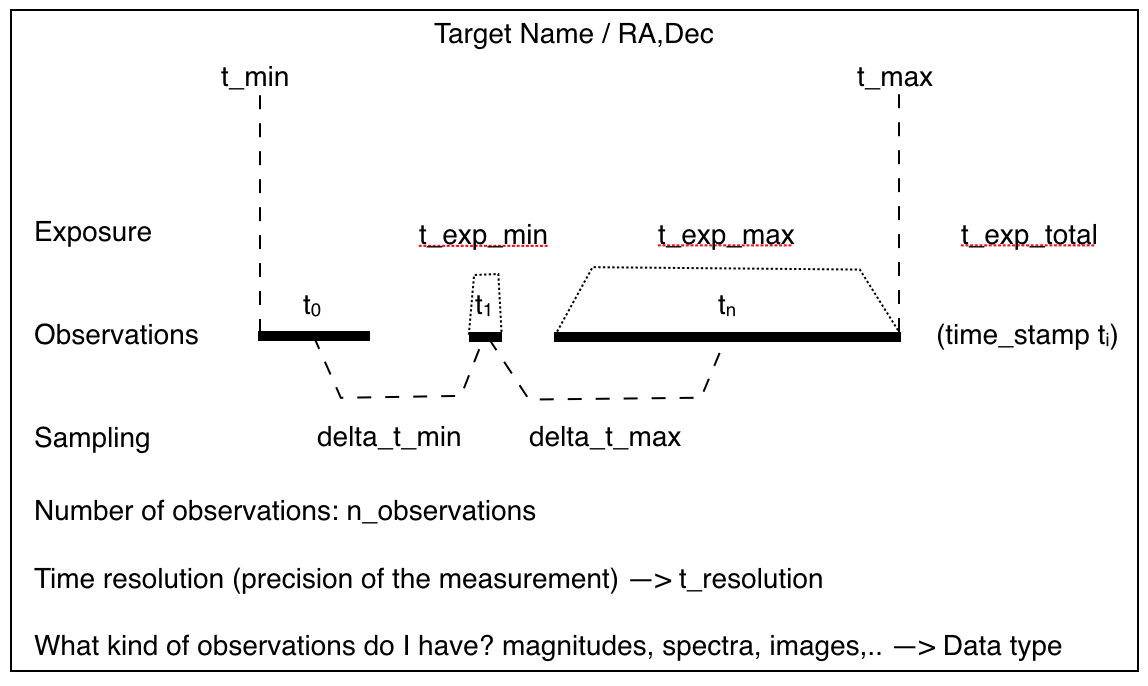
\includegraphics[width=0.8\textwidth]{figs/fig1.png}
\caption{Simple representation of Time Series data.} 
\label{fig:time-series}
\end{center}
\end{figure}

\begin{table}[hb] 
  \begin{center}
  \caption{Time Series metadata fields.}
  \label{tab:fields}
    \begin{tabular}{p{0.35\textwidth}p{0.64\textwidth}}
      \sptablerule
      \textbf{Field}  & \textbf{Explanation}                        \\\sptablerule
      (RA,Dec)        & Coordinates$^1$                             \\
      target\_name    & Target name$^1$                             \\ 
      t\_min          & Date of the begining of the time series  \\
      t\_max          & Date of the end of the time series          \\
      t\_exp\_min     & Minimum exposure time                       \\
      t\_exp\_max     & Maximum exposure time                       \\
      t\_exp\_total   & Total exposure time                         \\
      delta\_t\_min   & Minimum time sampling period / cadence             \\
      delta\_t\_max   & Maximum time sampling period/ cadence             \\
      t\_resolution   & Time resolution/precision                   \\
      n\_observations & Number of time integrations  in time series         \\
      type\_of\_data  & Type of data (fluxes, radial velocities, images,...)\\
      \sptablerule
    \end{tabular}
  \end{center}
  \textbf{Note:} $^1$For SSO or moving objects coordinates might not be enough or relevant. 
\end{table}

In many cases time series data is composed of only three columns: \emph{Time, Magnitude, Magnitude Error}.
This is the simplest kind of data set,  which is identified in the data product type vocabulary as 'light-curve'. 
See the IVOA product-type vocabulary at \url{https://www.ivoa.net/rdf/product-type/2024-03-22/product-type.html}.

For this data to be fully exploitable and reusable (interoperable) it has to be properly documented. In this specific case the minimum information that needs to be provided is: the object coordinates (or name), the filter in which the observations have been carried out, and the time frame and offset (if applicable).
However, the dimensionality of what is observed at the time stamps' sequence may correspond to 1D or 2D observations, like spectra or images  as well. 
That's why the dataproduct type  defined in ObsCore 1.1 should be more precise and eventually rely on the IVOA product-type vocabulary.

In addition, a mechanism should be defined to clarify what part of the data is varying with time, as described further in section \ref{sec:timevariant}. 

\subsection{Science use cases}
\label{sect:usecases}
Different science use cases for Time Series have been collected and described in by E. Solano  at \url{http://wiki.ivoa.net/twiki/bin/view/IVOA/CSPTimeSeries}. 
They highlight the case of optical light curves but can be generalized to all spectral regimes ( xray, gamma ray, radio, multi-messengers)  where time dependent measures have been taken.
Science cases are grouped according to their common requirements summarized as: 
\begin{itemize}
\item \textbf{Group A} Combine photometry and light curves of a given object/list of objects in the \emph{same} photometric band
\item \textbf{Group B} Combine photometry and light curves of a given object/list of objects in \emph{different} photometric bands
\item \textbf{Group C} Time series other than light curves
\end{itemize}

%\begin{table}
%  \begin{center}
%  \begin{tabular}{|l|l|l|l|l|l|}
%    \sptablerule
%    \bf{Science} & \bf{Target(s)} & \bf{Datatype} & \bf{Time} & \bf{Brightness} & \bf{Photometric} \\
%    \bf{Case}    &                &               &           &                 & \bf{Band}        \\\sptablerule
%    Group A      &  yes      &  lightcurves &  yes &    yes     &      one         \\
%    Group B      &  yes      &  lightcurves &  yes &    yes     &      several     \\
%    Group C      &  yes      &  time cubes, dynamic      &  yes &    no      &      no          \\
%    	&  & spectra, movie, etc &  &   &  \\ \sptablerule
%  \end{tabular}
%  \end{center}
%\end{table}
%

Looking at the different science cases we simplify the questions to two:
\begin{enumerate}
\item \emph{Have these two missions observed this object within these two dates?}
\item \emph{Is it possible to discover long/short term variability within the data?}

\end{enumerate}
To answer the first question a user needs to be sure that dates are comparable, that is time has to be brought into a common time frame. 
To answer the second question we need to keep track of the minimum and maximum time span. 

\subsection{Using a common time frame}
\label{sec:comtimeframe}
To compare datasets from different missions or archives a common representation of time is needed. In order to do so we propose to map time into a pivot format. Following \cite{2015A+A...574A..36R} and \cite{2007ivoa.spec.1030R} we propose a set of minimum metadata to be added for serializations of Time Series (see Table~\ref{tab:metadata}). 

\begin{table}[!htb] 
  \begin{center}
    \caption{Metadata for time in Time Series data serialisation.}
    \label{tab:metadata}
      \begin{tabular}{p{0.35\textwidth}p{0.64\textwidth}}
      \sptablerule
      \textbf{Parameter proposal} & \textbf{Explanation} \\\sptablerule
      t\_scale & Time frame scale is the scale used to measure time. IAU definition: "A time scale is simply a well defined way of measuring time based on a specific periodic natural phenomenon.''  See \url{http://aa.usno.navy.mil/publications/docs/Circular_179.pdf}. 
      Recognized time scale values and their meaning are listed in Table~\ref{tab:scales}. If we don't know use UNKOWN. \\
      t\_ref\_position &  Time Frame Position is the place where the time is measured. Standard values are listed in Table~\ref{tab:positions}. If we don't know use UNKOWN. \\
      t\_uncertainty & Resolution or uncertainty of the time stamps. \\
      t\_sys\_error  & Time Systematic Error to take into account our knowledge of the time frame (scale and position). If time\_scale is not known then 100s as DEFAULT value::, if t\_scale and t\_ref\_position are both not known then use  1000s as DEFAULT value. Approximately 100s is good for the time\_scale since that is related to changes in the clock in space/earth; 1000s is good if we do not know if times are corrected for the position of the Earth/satellite on its orbit around the Sun since that is approximately twice the time it takes the light to travel the Sun-Earth/satellite distance. \\
      t\_format  & Time representation as JD, MJD, ISO-8601. \\
      t\_offset &  Offset that has been subtracted to the time. Time can be relative to a certain moment, e.~g. time after the GRB that happened on date YYYYMMHHMMSS.SS or a random number the authors have subtracted from data to allow higher precision in the time stamps. Its default value is 0.0. \\
     t\_description & A text briefly describing what is varying with time. Photometric variability in filter V, Radial velocity curve in HJD. This field is aimed to help the reader. \\
    \sptablerule
    \end{tabular}
  \end{center}
\end{table}

We recommend to be specific on the time frame and we suggest to use:
\begin{center}
  JD(TT;BARYCENTER)
\end{center}
We also give some values that can be used as default in the case that some information is not known and impossible to recover. We minimize the impact of doing this by adding a systematic error to time when those values are unknown. 

\section{Extension of ObsCore}
ObsCore has a normalized description of the data content along the various physical axes where the data are projected. 
The spatial properties are described in the \emph{s\_*} group, the spectral ones in \emph{em\_*} group, the temporal ones in \emph{t\_*}, etc.
For each data set there is a minimal  set of metadata to describe its sky position, spectral band, time interval, etc. which are independent from each other.
This allows to enhance time sampling description by adding new parameters to the time group without putting the ObsCore existing model at risk. 

\subsection{Extension of ObsCore based on EPNCore}
Astronomy and space science both consider time series data and have proposed metadata data description for it. Some metadata have already been defined and used in the context of data discovery using ObsCore \cite{2017ivoa.spec.0509L}, and the remaining ones have been defined in the context of planetary data in the EPNcore specification \cite{2022ivoa.spec.0822E}. In Table~\ref{tab:obs_epn} we show the equivalence between the fields we require here and those existing in  ObsCore and EPNcore specifications. 

\begin{table}[!htb]  
  \begin{center}
  \begin{small}
  \caption{Equivalence and complementarity between Time Series data fields and ObsCore and EPNCore fields}
   \label{tab:obs_epn}
  \begin{tabular}{|l|l|l|}
%    \sptablerule
\hline
    \textbf{Field}      & \textbf{ObsCore field name} & \textbf{EPNCore field name}  \\%\sptablerule
\hline
    coordinates     & s\_ra, s\_dec          & -                         \\
    \hline
    target\_name    & target\_name           & target\_name              \\
    \hline
    t\_min          & t\_min                 & time\_min                 \\
    \hline
    t\_max          & t\_max                 & time\_max                 \\
    \hline
    t\_exp\_min     &  -                     & time\_exp\_min            \\
    \hline
    t\_exp\_max     &  -                     & time\_exp\_max            \\
    \hline
    t\_exp\_total   &  t\_exp                & -                         \\
    \hline
    delta\_min      &  -                     & time\_sampling\_step\_min \\
    \hline
    delta\_max      &  -                     & time\_sampling\_step\_max \\
    \hline
    n\_observations & t\_xel                 & -                         \\
    \hline
     t\_resolution   & t\_resolution      & -                         \\
%    \hline
    type\_of\_data  & dataproduct\_type & dataproduct\_type         \\
\hline
    %    \sptablerule
  \end{tabular}
  \end{small}

  \end{center}
 \end{table} 
 
\textbf{ Note:}  t\_resolution in ObsCore needs some clarification and the dataproduct\_type labels defined in ObsCore and EPNCore are different currently. 
That is why dataproduct\_type should be enriched in Obscore, and harmonized with the product type IVOA vocabulary maintained at \url{ivoa.net/rdf/}.

\subsection{Mentioning what part of the dataset varies with time }
\label{sec:timevariant}
Obscore 1.1 uses the attribute \emph{o\_ucd} to describe what is the quantity observed depending on the various physical axes of the data product. The  UCD string corresponding to the observable in  a one dimensional dataset is  easy to choose in the UCD list.  We propose to extend this definition to generalize for time series of multiple dimensional data sets and add a \emph{time\_variant} attribute in ObsCore.
In a time series, the principal axis considered is the Time axis. The time variant component can be either one dimensional, like for a light curve or velocity curve, or multi-dimensional. The time series is viewed as  time dependent sequence of components, which can be characterized  by a data product type, such as an image, a spectrum, a spectral cube, etc., also  defined in the product-type vocabulary. Table \ref{tab:timevar} summarizes the use of \emph{ time\_variant}  in various cases. 
This parameter is worth to include in the Time ObsCore extension table. 

\begin{table}[!htb]
   \begin{center}
  \caption{Time variant property of a temporally sampled dataset.  \label{tab:timevar} }
 
  \begin{small}
  \begin{tabular}{|l|l|l|}
\sptablerule
\textbf{Main dataproduct\_type} & \textbf{o\_ucd}  &\textbf{time\_variant}   \\ \hline
light curve & phot.flux &  scalar value \\ \hline
velocity curve & doppler.veloc & scalar value \\ \hline 
trajectory & pos.eq  &  sky position (vector) \\ \hline
dynamic spectrum & phot.flux & dp:spectrum \\ \hline
movie &   phot.flux & dp:image \\ \hline
time cube & phot.flux & dp:cube \\ \hline
 \end{tabular}
  \end{small}
  \end{center}
 \end{table} 
 
 \subsection{Time parameters defined in ObsCore v1.1}
 \label{sec:alreadythere}
 We have seen the data product type helps to search for time sampled data sets. 
 In order to describe properties of the data set along the time axis, we can reuse the axis properties defined in the Characterization data model \cite{2008ivoa.spec.0325L}.
 The idea is to describe how the time stamps are spanned along the time axis, with time duration and  cadence .
 \subsubsection{t\_min, t\_max}
 These parameters provide the bounds of the time coverage for this data set. For a light-curve it is the beginning of the first time sample and the end of the last sample.
  \subsubsection{t\_exptime}
  This parameter represents the duration or live time of the observation. 
  For a light-curve it is the sum of all valid time samples. For instance for a time-cube it is the total exposure time summing up all the poses.
  \subsubsection{t\_resolution}
  t\_resolution can be defined as the time limit under which two observable quantities cannot be distinguished from each other.
  This works for event-list, light-curve, time-cube data sets, etc. 
  \subsubsection{t\_xel, number of time stamps}
This parameter entails the number of observations in the time series. It is important to query for guessing how rich is the dataset, especially for observing variability .


%\begin{sidewaystable}
%\begin{tabular}...\end{tabular}
%\end{sidewaystable}

\begin{table}[!htb]

 \begin{flushleft}
  \caption{Definitions of Obscore time related attributes in the current specification.   \label{tab:timeinobscore} }
    \begin{scriptsize}
  \begin{tabular}{|l|l|l|l|l|} 
  \sptablerule
\textbf{Name}   & \textbf{Definition \&Utype} & \textbf{UCD} & \textbf{Units}& \textbf{Status} \\ \hline
\emph{t\_min}   & Time start of the sequence (MJD)  & time.start;obs.sequence & d &man\\ 
  & {\color{blue} Char.TimeAxis.Coverage.Bounds.Limits.LoLim} &   & & \\ \hline
\emph{t\_max} & Time end of the sequence & time.end;obs.sequence & d & man \\ 
 & {\color{blue}Char.TimeAxis.Coverage.Bounds.Limits.HiLim} & &  &  \\ \hline
\emph{t\_exptime}	&Exposure time (sum of multiple exposures)& time.duration;obs.exposure &s &man \\
 &	{\color{blue}Char.TimeAxis.Support.Extent} & &   & \\ \hline
\emph{t\_resolution} & Minimal interpretable time difference & time.resolution & s & man \\ 
 & {\color{blue}Char.TimeAxis.Resolution.Refval I}& & & \\ \hline 		
\emph{t\_xel}	&Number of time stamps in the series  & meta.number & null &	man\\ 
 & {\color{blue}Char.TimeAxis.numBins} & &  & \\ \hline 
 \end{tabular}
    \end{scriptsize}
 \end{flushleft}
\end{table}


 \section{Time parameters proposed for Obscore Extension }
 \label{sec:timeext}
 
  \subsection{Time Frame description}
  As mentioned in section \ref{sec:comtimeframe} the Time Frame description is essential for comparing various time series data sets .
This metadata was described first in the STC data model  \citep{2007ivoa.spec.1030R}, then  in the Coords DM \citep{2022ivoa.specQ1004R}, and serialized in the  VOTABLE format in the TimeSYS element .
Up to now, this metadata  was not defined in ObsCore1.1. It is coded into the VOTable  metadata of the dataset. 
Having  it as  part of the query response coming back for a search for time series would help the user application to interpret time stamps precisely.
MJD is the time format used for an ObsTAP query related to time. 
We propose to add the time frame parameters in the Time Obscore extension .
These various definitions are harmonized in the proposal given in  table \ref{tab:timereff}. We list the corresponding terms used in the Coords Data model and in the UCD vocabulary, as well as the attribute of the TIMESYS param defined for VOTable serialization. 
All terms are proposed optional, but they are highly recommended especially for new data collections. 

\begin{sidewaystable}[!htb]
\caption{ Time extension Table Summary. } %%%%%%%%%%%%%%%%%
\centering
 \subcaption{Time reference frame for searching and comparing temporally sampled datasets.   \label{tab:timereff}}
%
  \begin{small}
  \begin{tabular}{|l|l|l|l|l|l|l|}
\hline
t-obs  attribute& Definition & VODML-ID  & TIMESYS &UCD & Units&Status\\
 &  & in Coords DM &  attribute& & &\\  \hline
% Time Coordinate system						
{\color{blue}t\_origin} & Time frame origin & TimeOffset.time0 & timeorigin & time.epoch &  &	man	\\  \hline
{\color{blue}t\_scale} &	Time frame scale & TimeFrame.timeScale &timescale& time.scale &	?&man 	\\ \hline 
{\color{blue}t\_refPosition} &  Time reference position & TimeFrame.refPosition& refposition & & &man	\\  \hline 
{\color{blue}t\_refDirection} &Time reference direction&TimeFrame.refDirection&refdirection &	& & man 	\\ \hline 
%Time representation  ISOtime, MJD, JD, ?						
{\color{blue}t\_format}&	Time representation	& &  & time;meta.code.class&	null	&man	\\ \hline 
 
 \end{tabular}
 \bigskip
   \subcaption* {Sampling properties along Time axis. \label{tab:time_ext} }
\begin{tabular}{|l|l|l|l|l|l|}
 \hline
\bf{Name}   &	\bf{Definition} & \bf{Utype}&	\bf{UCD}	&\bf{Units}&	\bf{Status} \\ \hline
%
%
%{\color{blue}t\_origin} & Time frame origin & TimeOffset.time0  & time.epoch &  &	opt	\\  \hline
%{\color{blue}t\_scale} & Time frame scale & TimeFrame.timeScale & time.scale &	?&opt 	\\ \hline 
%{\color{blue}t\_refPosition} &  Time reference position & TimeFrame.refPosition & & &opt	\\  \hline 
%{\color{blue}t\_refDirection} &Time reference direction&TimeFrame.refDirection &	& & opt 	\\ \hline 
\hline
{\color{blue} t\_variant } & sub product attached to a time stamp &  & meta.code.class &  & opt\\ \hline
{\color{blue} t\_exp\_min} & minimal length of time sample & Char.TimeAxis.Sampling.Extent.loLim & time.duration; & s & man\\ 
&  (min integration time)& & obs.sequence;stat.min& & \\ \hline
{\color{blue}t\_exp\_max} & maximal length of time sample  & Char.TimeAxis.Sampling.Extent.hiLim & time.duration; & s & man\\ 
& (max integration time) & &bs.sequence;stat.max & & \\ \hline
%time space between 2 time samples / cadence					
{\color{blue}t\_delta\_min} & minimal length of time interval & Char.TimeAxis.Sampling.Period.loLim & time.interval; & s & man \\ 
& cadence (min)& &obs.sequence;stat.min  & &   \\ \hline
{\color{blue}t\_delta\_max} & maximal length of time interval & Char.TimeAxis.Sampling.Period.hiLim & time.interval;& s & man\\ 
& cadence (max)& & obs.sequence;stat.max& &  \\ \hline
{\color{blue} t\_fold\_period}& Folding period length &  & time.period&d & opt  \\ \hline
{\color{blue} t\_fold\phaseReference}& Folding convention: phase reference &  & meta.ref;time.phase&d & opt  \\ \hline

 \end{tabular}

  \end{small}
 \end{sidewaystable} 
 
 
Values to fill these terms should rely on the terms defined in IVOA vocabularies, namely for  time scales and time reference position. 
As an example Appendix A summarize the definitions listed in previous models like STC.
 
\subsection{Time axis sampling description}
\emph{t\_delta\_min }, \emph{t\_delta\_max}  represent the minimal (resp. maximal) time interval between two time samples.
This concept is covered in the Characterization data model \citep{2008ivoa.spec.0325L} and designated as sampling period along the Time axis. 
The cadence of the observations in the time series  can be assumed from theses parameters. 
 
 The Time Axis Sampling Extent defined in Characterization DM is the duration of each sample and may vary along the time sequence. 
 During the observation process, it corresponds to an exposure time. 
 If the sampling is not regular the minimal and maximal value described in \emph{ t\_exp\_min, t\_exp\_max} can be used. 
When the sampling extent  is even, all samples have the same duration and  t\_exp\_min, t\_exp\_max have the same value. 
When the sampling period, or cadence  is even, \emph{t\_delta\_min }, \emph{t\_delta\_max} have the same value. 
% ZTF ? LSST? typical values? 

\subsection{Time axis mode and folding period }
Time series may be distributed in two modes, "search mode" or "folded". 
The folding allows to improve the SNR and to analyse further the periodicity of the observed phenomenon.
For data discovery  purpose one parameter may be introduced : \emph{t\_fold\_period}, the time duration of the folding .
A \emph{t\_fold\_period} parameter set to zero means not folded  and clarifies in which mode are the data. 
% 
% \begin{sidewaystable}[!htb] 
% % \begin{center}
%  \caption{Table of  Obscore Time extension  attributes, \\ Here are the extended features for comparing time sampled data sets.\label{tab:time_ext}}
%   \begin{small}
%  \begin{tabular}{|l|l|l|l|l|l|}
% \hline
%\bf{Name}   &	\bf{Definition} & Utype&	UCD	&Units&	Status \\ \hline
%t\_variant  & datatype of the leaf data set of time stamps &  & meta.code.class &  & opt\\ 
%&  (min integration time)& & & & \\ \hline
% t\_exp\_min & minimal length of time sample & Char.TimeAxis.Sampling.Extent.loLim & time.duration; & s & opt\\ 
%&  (min integration time)& & obs.sequence;stat.min& & \\ \hline
%t\_exp\_max & maximal length of time sample  & Char.TimeAxis.Sampling.Extent.hiLim & time.duration; & s & opt\\ 
%& (max integration time) & &bs.sequence;stat.max & & \\ \hline
%%time space between 2 time samples / cadence					
%t\_delta\_min & minimal length of time interval & Char.TimeAxis.Sampling.Period.loLim & time.interval; & s & opt \\ 
%& cadence (min)& &obs.sequence;stat.min  & &   \\ \hline
%t\_delta\_max & maximal length of time interval & Char.TimeAxis.Sampling.Period.hiLim & time.interval;& s & opt \\ 
%& cadence (max)& & obs.sequence;stat.max& &  \\ \hline
%t\_fold\_period& Folding period length &  & time.period&d & opt  \\ \hline
% \end{tabular}
%   \end{small}
% % \end{center}
% \end{sidewaystable} 

 \section{Extension mechanism in ObsTAP }
 \label{sec:comext}
 ObsCore is mostly implemented in the TAP protocol \citep{2019ivoa.spec.0927D}.
 % note:TSSerialisationNote
 An ObsTAP service is considered compliant to the standard if it serves all the attributes tagged as mandatory in the specification.
 These are gathered in the TAP\_SCHEMA in the table usually named \emph{ivoa.obscore}. 
 Following the practice introduced  for EPNTap,  the utype column in \emph{ivoa.obscore} should be the standard identifier of the specification supported by the table content, so here \texttt{ivo://ivoa.net/std/obscore\#table-1.1}
 
 This table can also hold more columns corresponding to  optional attributes, as summarized in the Table 7 - Optional Parameters  of the ObsCore specification.
 There is no guarantee that an optional parameter will be filled in an ObsTAP service; this must be checked first by the user. 
 
 Therefore the Time extension for Obscore should rely on mandatory parameters. 
 They may be set UNKNOWN if unknown.
 In order to warn users that extra time parameters have been included in ObsTAP, we propose to gather them  in another table named \emph{ivoa.t-obs}
 for services that distribute time sampled data sets. 
 The utype column in  \emph{ivoa.t\_obs} should be the standard identifier of this specification, so here \texttt{ivo://ivoa.net/std/obscore\#t-obs-1.0}.

 If this table contains an identifier for the corresponding dataset described in main \emph{ivoa.obscore} table, then it is easy to join  general Obscore properties to the time specific ones in an ADQL query.
 Here is a query  example :  ( to be checked) 
 \begin{lstlisting} [language=SQL, caption= Query example for Join between the main ObsCore table and the Time extension table]
 SELECT obs_id, t_min, t_max, obs_publisher_did, obs_collection, access.reference FROM ivoa.obscore 
 WHERE dataproduct_type=='light-curve'
 AND t_min > 55197 
 AND t_max < 55204
 JOIN ivoa.t-obs as tt
 ON obs_publisher_did==tt.obs_publisher_did
  WHERE tt.delta_min < 10s AND  tt.t_xel > 10
 \end{lstlisting}

Other examples of queries using these extra parameters are proposed in Appendix \ref{sec:query_examples}.

More generally, other extensions can be considered in ObsTAP, like the radio extension or high energy extension specific to these spectral domains and instrumentations. 
In an extended OBSTAP service the main Obscore table and the other extension tables must be gathered in a TAP\_SCHEMA with utype  \texttt{ivo://ivoa.net/std/obscore1.1}, for version 1.1 and containing the different tables : ivoa.obscore, ivoa.t-obs, ivoa.radio, ivoa.heig etc....
This would guarantee that all the tables for data discovery are grouped together and discovered, and that the service can be joined.
% exemples of joins

%SELECT TOP 10 lat, long, flux 
%FROM lightmeter.measurements 
%JOIN lightmeter.stations
%USING (stationid)

  
\appendix

\section{Recognized time scales }
\label{appendix1}
\begin{table}
  \begin{center}
    \caption{Recognized time scale values. \\ Table reference for time scales :  Table 2, p17 in Space-Time Coordinate Metadata for the Virtual Observatory
Version 1.33}\label{tab:scales}
      \begin{tabular}{p{0.15\textwidth}p{0.84\textwidth}}
      \sptablerule
      \textbf{Parameter} & \textbf{Explanation} \\\sptablerule
TAI   & (International Atomic Time) atomic time standard maintained on the rotating geoid\\
TT    & (Terrestrial Time; IAU standard) defined on the rotating geoid, usually derived as TAI + 32.184 s\\
TDT   & (Terrestrial Dynamical Time) synonym for TT (deprecated)\\
ET    & (Ephemeris Time) continuous with TT; should not be used for data taken after 1984-01-01 \\
IAT   & synonym for TAI (deprecated) \\
UT1   & (Universal Time) Earth rotation time \\
UTC   & (Universal Time, Coordinated; default) runs synchronously with TAI, except for the occasional insertion of leap seconds intended to keep UTC within 0.9 s of UT1; as of 2012-07-01 UTC = TAI - 35 s \\
GMT   & (Greenwich Mean Time) continuous with UTC; its use is deprecated for dates after 1972-01-01\\
UT()  & (Universal Time, with qualifier) for high-precision use of radio signal distributions between 1955 and 1972; see Sect. A.9 \\
GPS   & (Global Positioning System) runs (approximately) synchronously with TAI; GPS $\approx$ TAI - 19 s\\
TCG   & (Geocentric Coordinate Time) TT reduced to the geocenter, corrected for the relativistic effects of the Earth’s rotation and gravitational potential; TCG runs faster than TT at a constant rate.\\
TCB   & (Barycentric Coordinate Time) derived from TCG by a 4-dimensional transformation, taking into account the relativistic effects of the gravitational potential at the barycenter (relative to that on the rotating geoid) as well as velocity time dilation variations due to the eccentricity of the Earth’s orbit, thus ensuring consistency with fundamental physical constants; Irwin \& Fukushima (1999) provide a time ephemeris.\\
TDB   & (Barycentric Dynamical Time) runs slower than TCB at a constant rate so as to remain approximately in step with TT; runs therefore quasi-synchronously with TT, except for the relativistic effects introduced by variations in the Earth’s velocity relative to the barycenter; when referring to celestial observations, a pathlength correction to the barycenter may be needed which requires the Time Reference Direction used in calculating the pathlength correction.\\
LOCAL & for simulation data and for free-running clocks.\\
    \sptablerule
      \end{tabular}
%      \textbf{Notes.}
%      $^{(1)}$ Specific realizations may be appended to these values, in parentheses; see text. For a more detailed discussion of time scales, see Appendix A.
%      $^{(2)}$ Recognized values for TIMESYS, CTYPEia, TCTYPn, TCTYna.
  \end{center}
\end{table}


\begin{table}
  \begin{center}
    \caption{Recognized time reference positions. Table reference for time position : Table 1, p15 in Space-Time Coordinate Metadata for the Virtual Observatory
Version 1.33, \url{https://www.ivoa.net/documents/REC/DM/STC-20071030.pdf} }\label{tab:positions}
      \begin{tabular}{p{0.25\textwidth}p{0.74\textwidth}}
      \sptablerule
      \textbf{Parameter} & \textbf{Explanation} \\\sptablerule
TOPOCENTER  &	Topocenter: the location from where the observation was made (default)\\
GEOCENTER   &	Geocenter\\
BARYCENTER  &	Barycenter of the Solar System\\
RELOCATABLE &	Relocatable: to be used for simulation data only\\
CUSTOM	    & A position specified by coordinates that is not the observatory location\\
%Less common allowed standard values are:\\
HELIOCENTER & 	Heliocenter\\
GALACTIC    &	Galactic center\\
EMBARYCENTER&	Earth-Moon barycenter\\
MERCURY	    & Center of Mercury\\
VENUS	    & Center of Venus\\
MARS	    & Center of Mars\\
JUPITER	    & Barycenter of the Jupiter system\\
SATURN	    & Barycenter of the Saturn system\\
URANUS	    & Barycenter of the Uranus system\\
NEPTUNE	    & Barycenter of the Neptune system\\
          \sptablerule
      \end{tabular}
      \end{center}
\end{table}

  


\appendix 
\label{sec:query_examples}

\section{Query examples for join tables}
\appendix
\section{Previous work on the Time series characterization and description}. 

\begin{itemize}  
\item Very initial draft initiated by D. Tody
\url{https://wiki.ivoa.net/internal/IVOA/LightCurves/STSP.pdf}
\item Table reference for time position : Table 1, p15 in Space-Time Coordinate Metadata for the Virtual Observatory
Version 1.33, \url{https://www.ivoa.net/documents/REC/DM/STC-20071030.pdf} 
\item Table reference for time scales :  Table 2, p17 in Space-Time Coordinate Metadata for the Virtual Observatory
Version 1.33
\item 
\end{itemize} 

\section{Vocabulary enhancement}
 \url{https://www.ivoa.net/rdf/product-type/2024-03-22/product-type.html}
has evolved to clarify the various temporally-sampled datasets and their class. \\
light-curve, velocity-curve, dynamic-spectrum, time-cube clarifies categories of time dependent data sets .

\section{Changes from Previous Versions}

First version of this WD. 
No previous versions yet.
% these would be subsections "Changes from v. WD-..."
% Use itemize environments.


% NOTE: IVOA recommendations must be cited from docrepo rather than ivoabib
% (REC entries there are for legacy documents only)
\section{References}
\bibliography{ivoatex/ivoabib, ivoatex/docrepo, ivoatex/myref}
 % note:TSSerialisationNote
 

\end{document}
